%!TEX root = ../aufgabenstellung.tex

\section{Entwurf \enquote{Roboter im Straßenverkehr} \points{46}}

Gegeben ist ein Straßenverkehrssystem mit einem rasterförmigen Netz von horizontalen und vertikalen Straßen.
An jeder Kreuzung befinden sich Ampeln, die den Verkehrsfluss steuern.

\begin{center}
	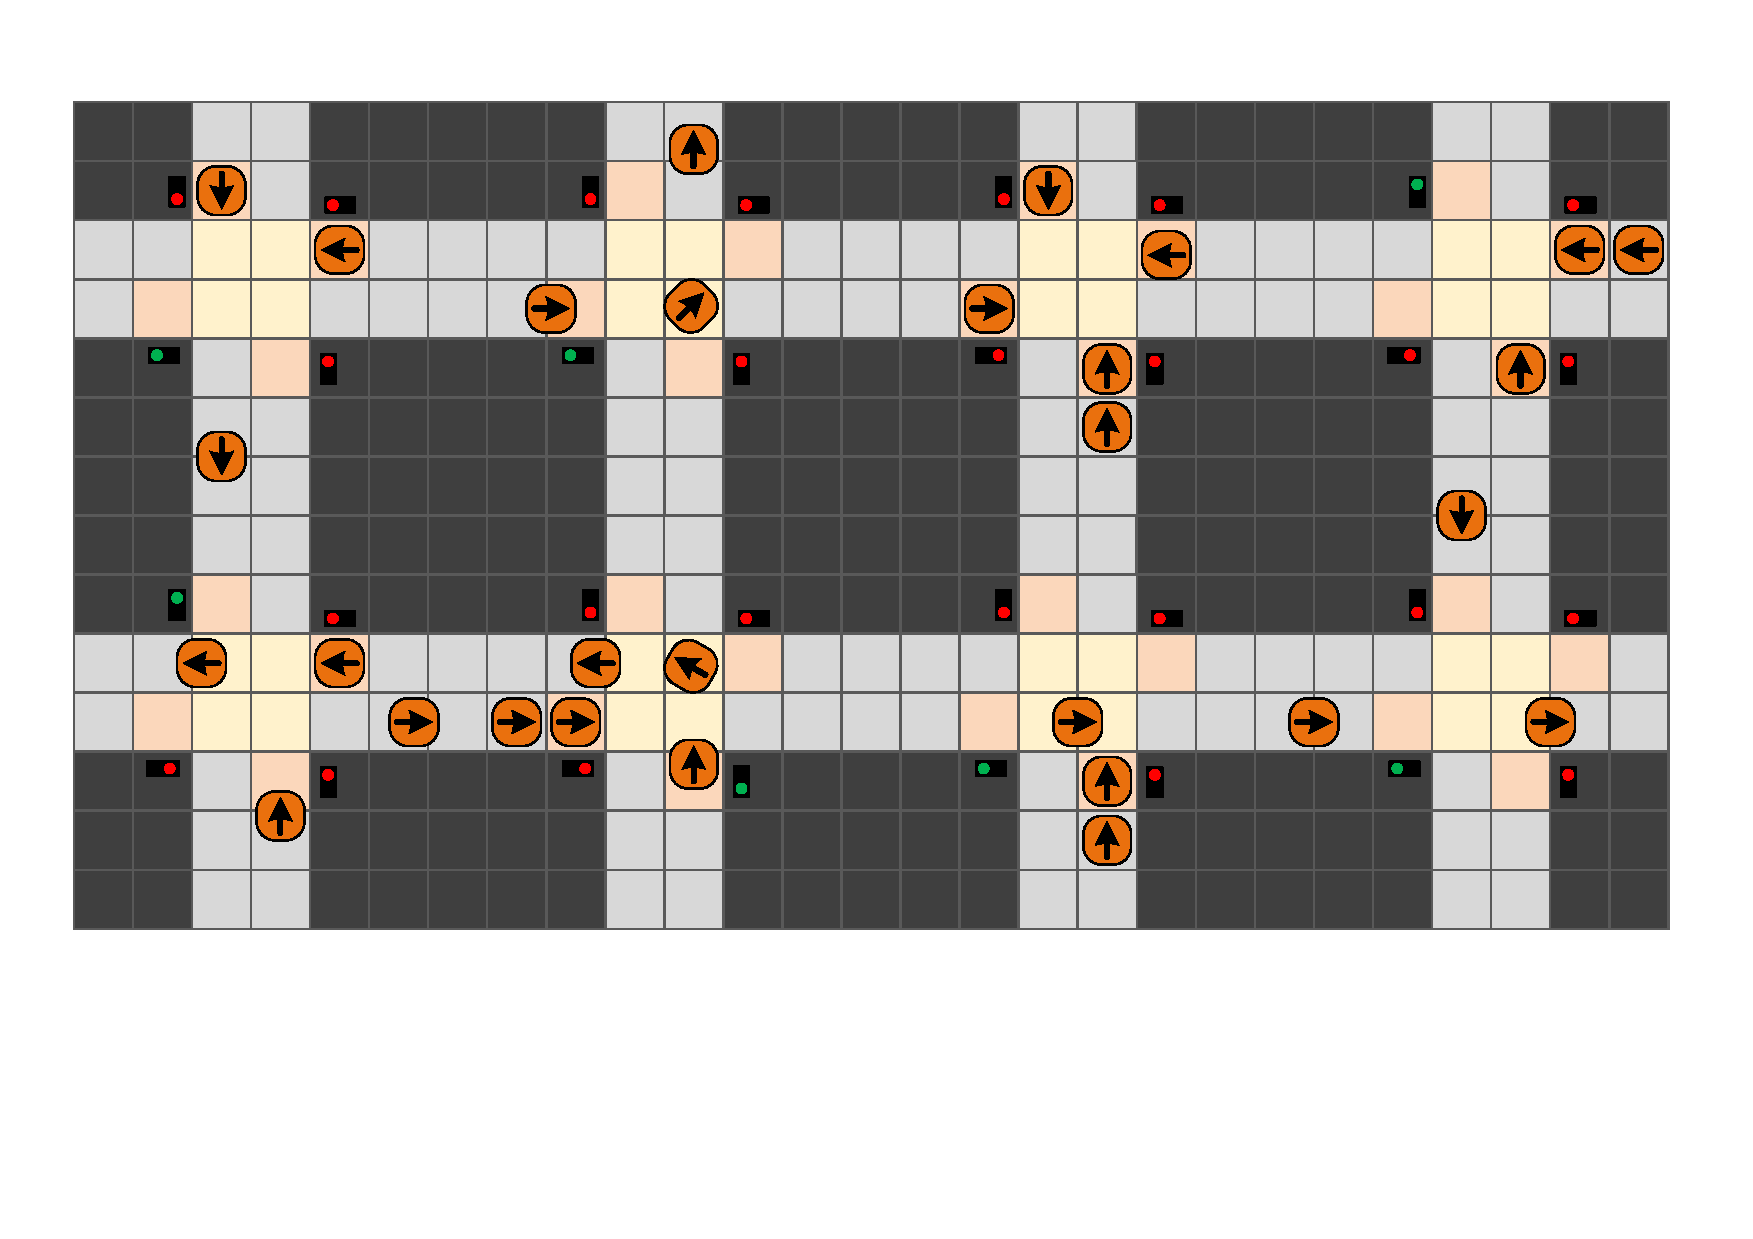
\includegraphics[width=.8\textwidth]{verkehr_skizze.pdf}
\end{center}

In diesem auf einzelne Felder aufgeteilten, zweidimensionalen Straßennetz fahren autonome Roboter zu von einem zentralen Server vorgegebenen Zielen.
Die Roboter fahren im Rechtsverkehr (d.h. immer auf der in Fahrtrichtung gesehen rechten Spur) und achten beim Fahren autonom darauf, dass sie 
\begin{enumerate*}
 	\item nicht auf andere Roboter auffahren,
 	\item die Ampelzeichen beachten und 
 	\item an Kreuzungen passend abbiegen.
 \end{enumerate*} 

In dieser Aufgabe soll die Steuerungssoftware der Roboter, konkret die aktive Klasse \texttt{RobotControl}, implementiert werden. Für die Software der Roboter ist folgendes Klassendiagramm gegeben:

\begin{center}
	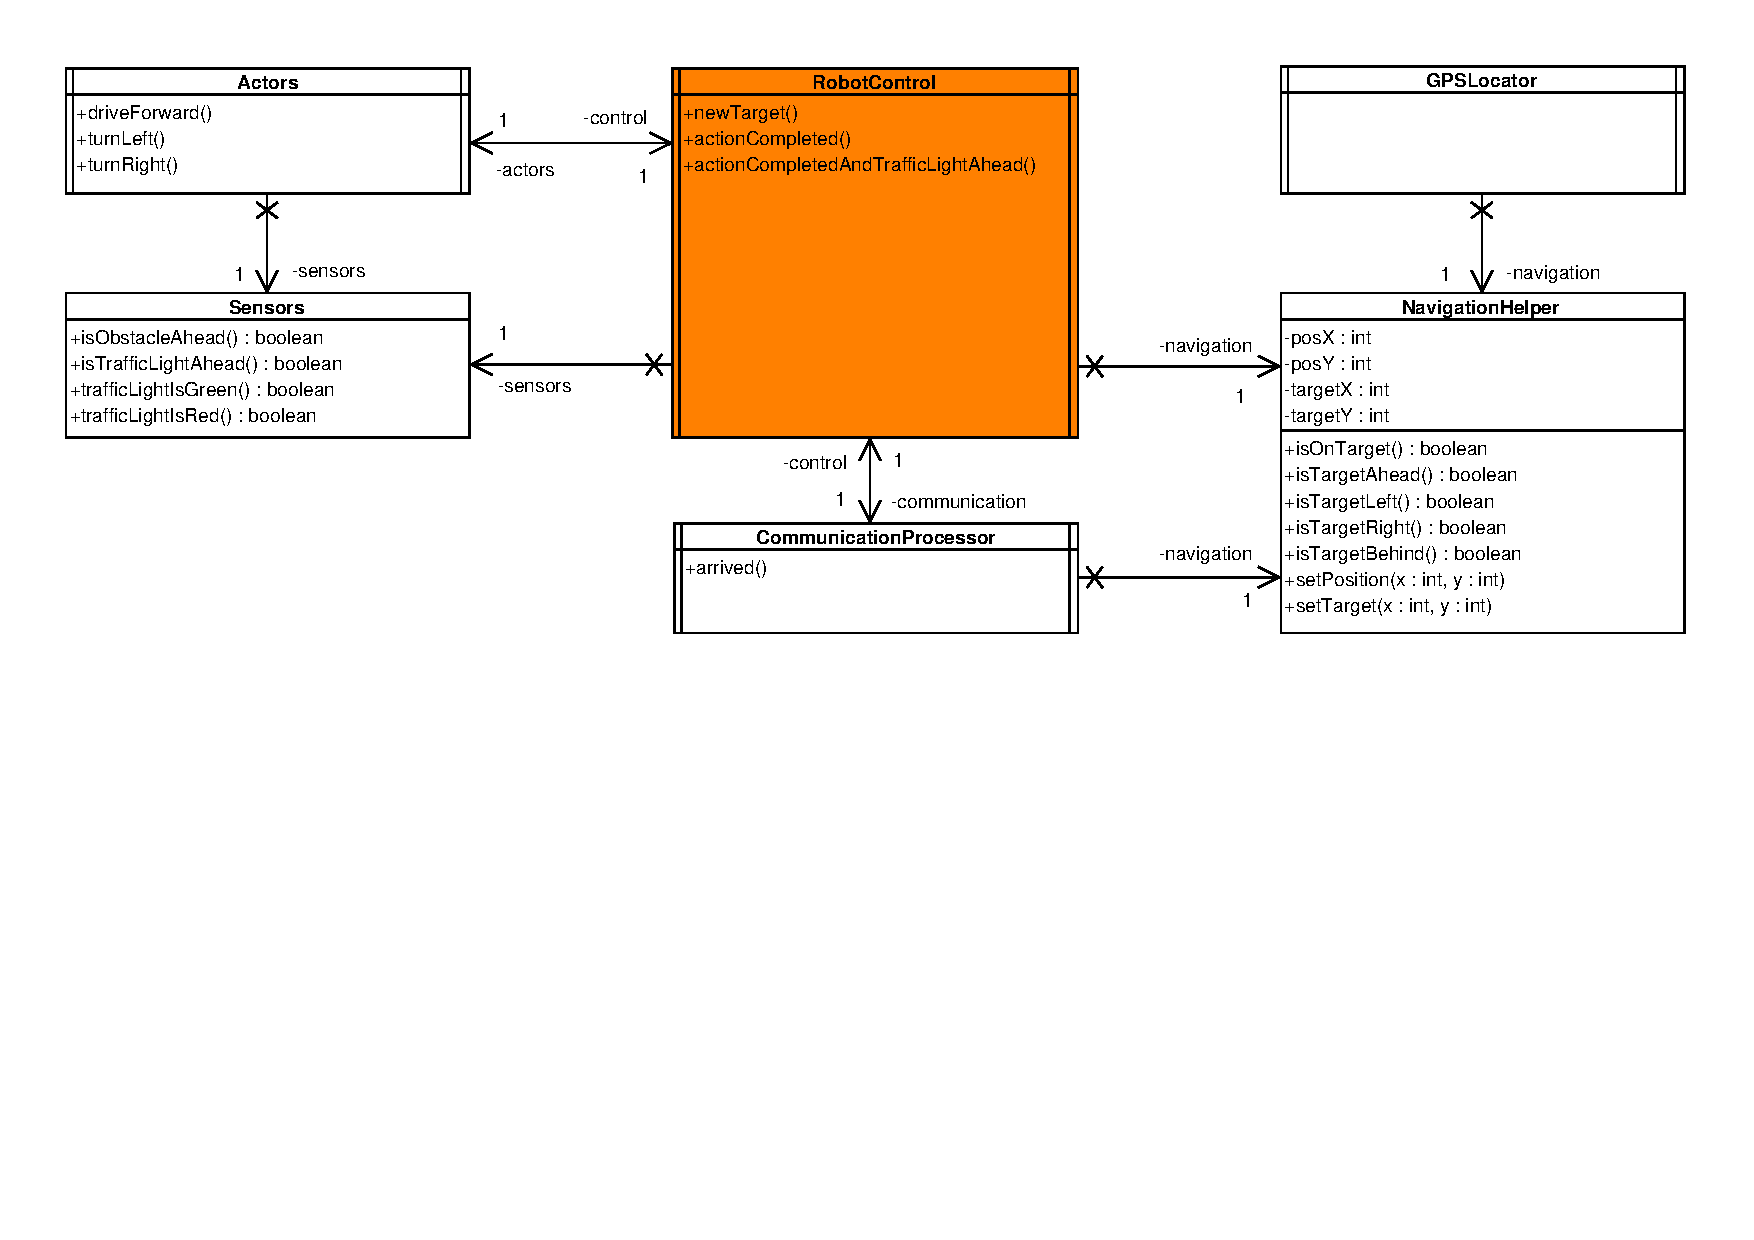
\includegraphics[width=1\textwidth]{verkehr_roboter_klassendiagramm.pdf}
\end{center}


Ein Roboter ist zu Beginn pausiert.
Im weiteren Verlauf ist er immer entweder pausiert oder hat ein bestimmtes Fahrziel, das ihm vom zentralen Server zugewiesen wird und zu dem er fährt.
Wenn ein neues Ziel beim \texttt{CommunicationProcessor}-Objekt ankommt, setzt dieses mit der Methode \texttt{setTarget(x,y)} den \texttt{NavigationHelper} über die neuen Koordinaten in Kenntnis und informiert das \texttt{RobotControl}-Objekt mit dem Methodenaufruf \texttt{newTarget()}.
Es kann angenommen werden, dass weder die Startposition des Roboters bei Erhalt eines Auftrags noch dessen Ziel jemals auf einer Kreuzung oder auf einem Feld direkt vor oder direkt hinter einer Kreuzung liegt.
Außerdem ist das Ziel niemals gleich der Startposition. 

Wenn ein Roboter ein Ziel hat fährt er, solange das Ziel noch nicht erreicht ist, Feld für Feld geradeaus entlang der Straßen, und nutzt ggf. die Kreuzungen, um nach links oder rechts abzubiegen. 
Nach jeder Aktion, bei der er potentiell das Ziel erreicht haben könnte, wird dies mit der Abfrage \texttt{isOnTarget()} beim \texttt{NavigationHelper} überprüft.

Um Kollisionen zu vermeiden ruft das \texttt{RobotControl}-Objekt vor jeder Aktion, bei der es notwendig ist, die Methode \texttt{isObstacleAhead()} beim \texttt{Sensors}-Objekt auf. Wenn die Methode \texttt{true} zurückgibt bedeutet das, dass das nächste Feld in Fahrtrichtung bereits mit einem Roboter belegt ist. Das \texttt{RobotControl}-Objekt muss dann solange immer wieder die Sensoren abfragen, bis das Feld frei geworden ist.

Eine Aktion eines Roboters ist immer entweder die Bewegung um ein Feld vorwärts in Fahrtrichtung, das Drehen auf der Stelle nach links oder das Drehen auf der Stelle nach rechts. Diese Aktionen werden vom \texttt{RobotControl}-Objekt jeweils mit den Methoden \texttt{driveForward()}, \texttt{turnLeft()} und \texttt{turnRight()} beim \texttt{Actors}-Objekt aufgerufen.
Wenn die entsprechende Aktion abgeschlossen ist, meldet das \texttt{Actors}-Objekt dies mit dem Aufruf \texttt{actionCompleted()} an das \texttt{RobotControl}-Objekt zurück, welches dann die nächste Aktion aufrufen kann.

Das \texttt{Actors}-Objekt ruft zudem nach jedem Vorwärtsfahren die Methode \texttt{isTrafficLightAhead()} beim \texttt{Sensors}-Objekt auf, um festzustellen, ob die Warteposition vor einer Ampel erreicht wurde. Wenn dies der Fall ist, wird beim \texttt{RobotControl}-Objekt statt \texttt{actionCompleted()} die Methode \texttt{actionCompletedAndTrafficLightAhead()} aufgerufen.

Wenn ein Roboter vor einer Ampel steht muss er warten, bis diese grün ist. Dazu wird wiederholt \texttt{trafficLightIsGreen()} oder \texttt{trafficLightIsRed()} beim \texttt{Sensors}-Objekt abgefragt. 
Sobald die Ampel grün zeigt kann die Kreuzung befahren werden und geradeaus, nach links oder nach rechts verlassen werden, wobei das Durchfahren der Kreuzung immer aus einer Sequenz von mehreren, beim \texttt{Actors}-Objekt aufgerufenen Einzelaktionen besteht. 
Es kann davon ausgegangen werden, dass die Ampel nur Roboter aus einer Richtung einfahren lässt, sodass links abbiegende Roboter kein Problem mit Gegenverkehr haben. 

Um festzustellen, in welche Richtung der Roboter auf der Kreuzung fahren muss, stellt das \texttt{NavigationHelper}-Objekt die Methoden \texttt{isTargetAhead()}, \texttt{isTargetLeft()} und \texttt{isTargetRight()} bereit, die jeweils einen \textt{boolean} zurückgeben. Die Methoden funktionieren zuverlässig sowohl bei einer Roboter-Position vor als auch auf einer Kreuzung. Es ist möglich, dass mehrere dieser Methoden in einer Situation \texttt{true} ergeben.

Wenn der Roboter sein Ziel erreicht hat pausiert er sofort und meldet die Ankunft mit dem Aufruf \texttt{arrived()} an den \texttt{CommunicationProcessor}.
Das \texttt{RobotControl}-Objekt pausiert bis es einen neuen \texttt{newTarget()}-Aufruf erhält.






\begin{enumerate}[a) ]
	\item Modellieren Sie die Struktur der beschriebenen Robotersteuerungssoftware für \textit{einen} Roboter mit einem Objektdiagramm. Der Roboters ist an Position \texttt{x=8}, \texttt{y=14}, das Ziel ist \texttt{x=10}, \texttt{y=16}.
	Achten Sie auf Konsistenz zum vorgegebenen Klassendiagramm. \points{8}
\end{enumerate}

\solutionbox{
	\red{Musterlösungen sind nicht öffentlich, können aber auf Anfrage bereitgestellt werden.}
}

\solution{\newpage}















\begin{enumerate}[a) ,resume]
	\item Modellieren Sie das Verhalten der aktiven Klasse \texttt{RobotControl} mit einem Zustandsdiagramm.
	Stellen Sie insbesondere sicher, dass Ihr Zustandsdiagramm ein sicheres Fahrverhalten realisiert, sodass die Roboter 
	\begin{enumerate*}[1. ]
	 	\item nicht auf andere Roboter auffahren,
	 	\item die Ampelzeichen beachten und 
	 	\item an Kreuzungen passend abbiegen.
	 \end{enumerate*} 

	In Situationen, in denen regelmäßig eine Abfrage erfolgen muss (z.B. beim Warten auf eine grüne Ampel), verwenden Sie \texttt{after 100ms} als Trigger und \underline{nicht} den Trigger \texttt{when}.

	Achten Sie auf Konsistenz zum vorgegebenen Klassendiagramm. \points{24}
	
	\fbox{\parbox{0.95\textwidth}{
		\textbf{Hinweis:} Nutzen Sie für diese Teilaufgabe die YAKINDU Statechart Tools für die Modellierung. Laden Sie bei der Abgabe neben der üblichen PDF-Datei ein \texttt{.zip}-Archiv im Moodle hoch, welches die \texttt{simpletraffic\_robot.ysc}-Datei mit Ihren Diagramm enthält.
		\newline
		\newline
		Wir stellen Ihnen für diese Übung ein Framework zur Verfügung, mit dem Sie das durch ihr Zustandsdiagramm definierte Fahrverhalten der Roboter selbst erproben und beobachten können.
		Weitere Informationen zur Installation  und Verwendung der YAKINDU Statechart Tools und des Simulators finden Sie in dem im Moodle hinterlegten Dokument \texttt{\red{Toolhinweise.pdf}}. 
		\newline
		\newline
		Beachten Sie, dass die Diagramm-Syntax in den YAKINDU Statechart Tools von der üblichen UML-Syntax abweicht. Die wichtigsten Besonderheiten sind ebenfalls in \texttt{\red{Toolhinweise.pdf}} kurz aufgelistet. Für die Klausur müssen Sie nur die Syntax von UML-Zustandsdiagrammen beherrschen.
	}}
\end{enumerate}


\solutionbox{
	\red{Musterlösungen sind nicht öffentlich, können aber auf Anfrage bereitgestellt werden.}
}

\solution{\newpage}






\begin{enumerate}[a) ,resume]
	\item Modellieren Sie die Interaktion zwischen den Objekten der Robotersteuerungssoftware bei dem folgenden beispielhaften Ablauf mit einem Sequenzdiagramm:


    \begin{minipage}{.7\textwidth}
    	Der Roboter ist initial pausiert. Die initiale Position ist \texttt{x=8}, \texttt{y=14}. 
		%
		Der \texttt{CommunicationProcessor} erhält vom zentralen Server den Auftrag, zur Position \texttt{x=10}, \texttt{y=16} zu fahren und gibt diesen Befehl entsprechend weiter.
		%
		Es werden keine anderen Roboter oder sonstige Hindernisse auf der Strecke angetroffen.
		Beim Erreichen der Ampel ist diese bei der ersten Abfrage der Sensoren rot, aber bereits bei der zweiten Abfrage grün.
		%
		Nach Ankunft am Ziel meldet der Roboter dies über den \texttt{CommunicationProcessor} an den zentralen Server. Es folgen keine weiteren Fahrbefehle. Der Ablauf ist damit beendet.
    \end{minipage}
    \begin{minipage}{.25\textwidth}
		\begin{center}			
	    	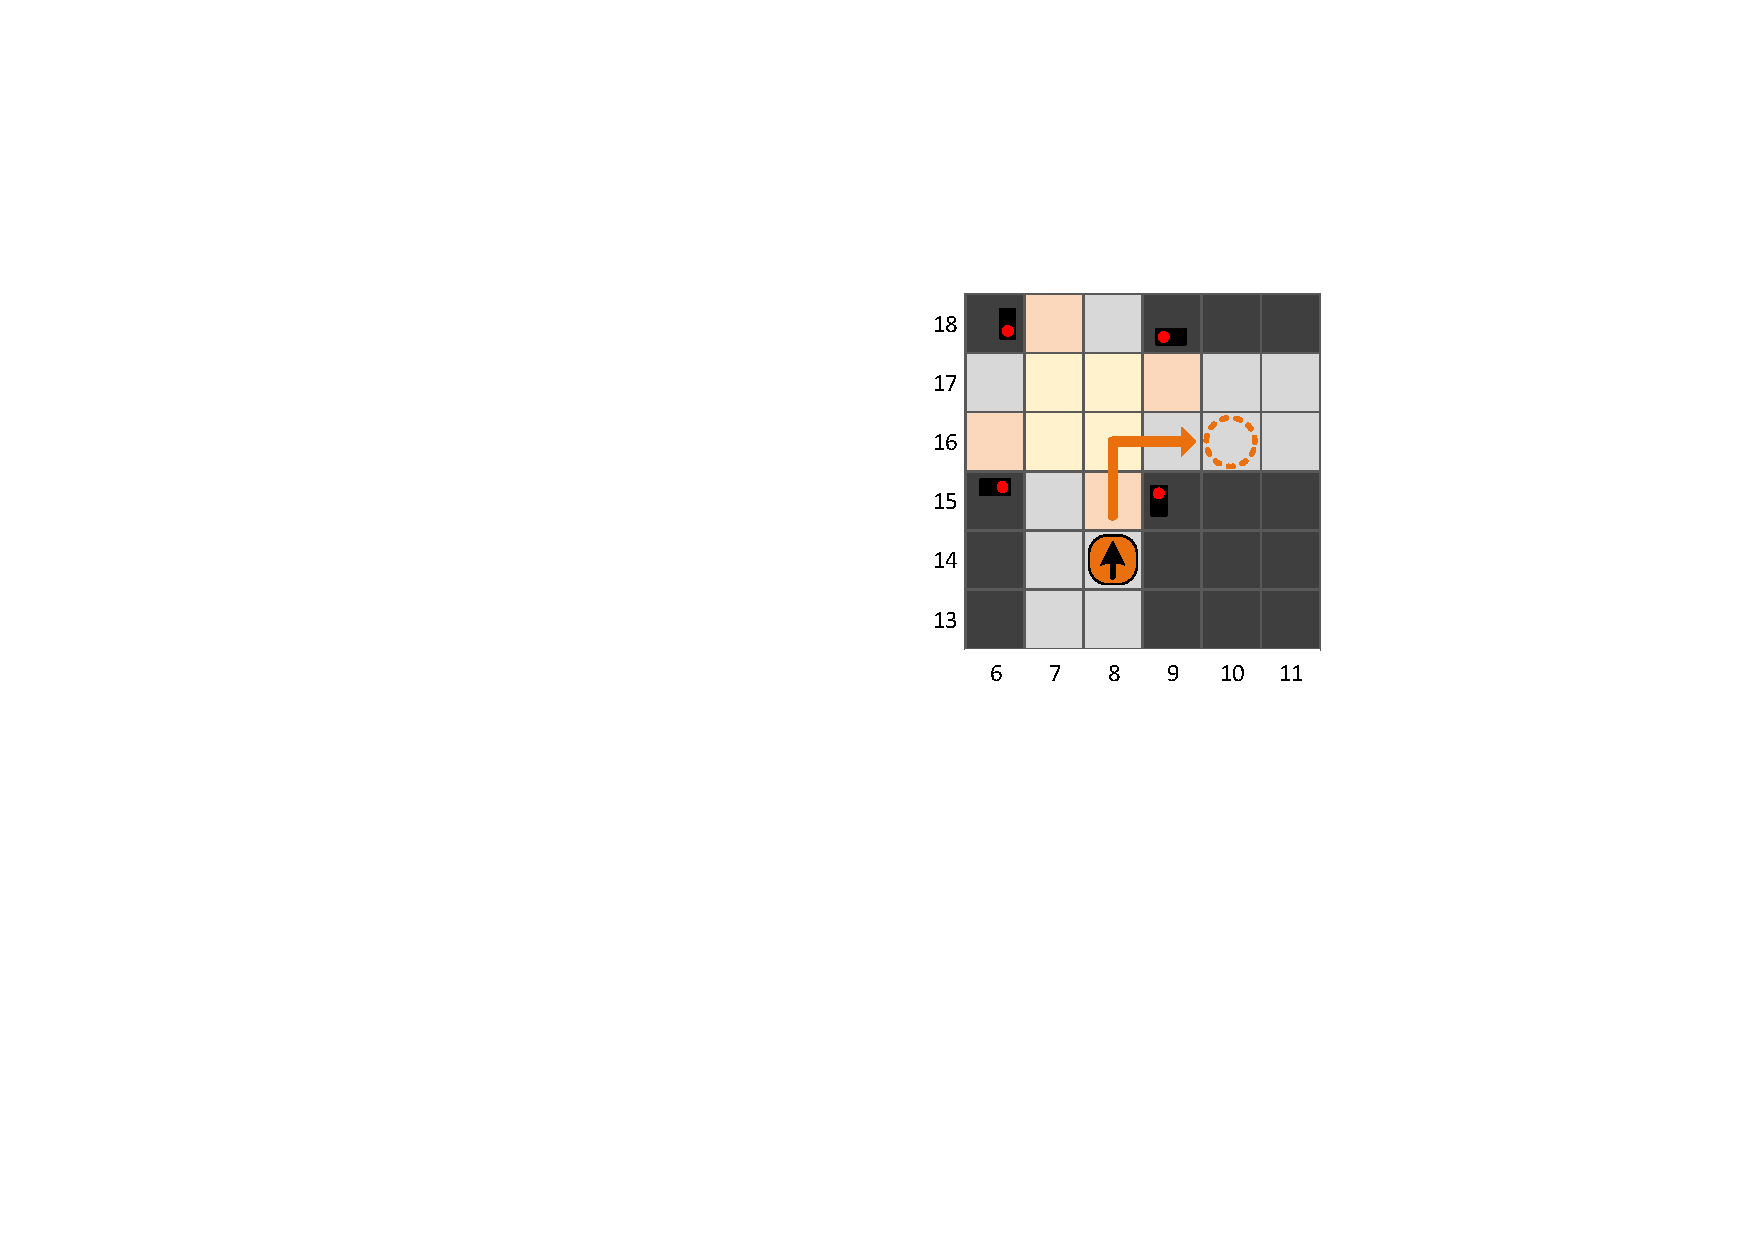
\includegraphics[width=0.9\textwidth]{verkehr_roboter_beispielablauf.pdf}
		\end{center}			
    \end{minipage}

	Modellieren Sie nur die Interaktion der Objekte der Klassen \texttt{RobotControl}, \texttt{Actors}, \texttt{Sensors}, \texttt{CommunicationProcessor} und \texttt{NavigationHelper}.
	Das Objekt der Klasse \texttt{GPSLocator} sowie der zentrale Server müssen \underline{nicht} beachtet werden.

	Verwenden Sie in den Aufrufen konkrete Werte als Parameter oder Rückgabewert.
%
	Achten Sie bei der Modellierung auf Konsistenz zum vorgegebenen Klassendiagramm und zu Ihrem UML-Zustandsdiagramm aus Teilaufgabe b). \points{14}

\end{enumerate}


\solutionbox{
	\red{Musterlösungen sind nicht öffentlich, können aber auf Anfrage bereitgestellt werden.}
}
